\documentclass[../main/main.tex]{subfiles}

\newdate{date}{16}{04}{2020}

\begin{document}

\section{Lecture 12}
 \displaydate{date}. Compiled:  \today. Martina.

\subsubsection{Slide 196}

\begin{figure}[h!]
\centering
\includegraphics[page=18,width=0.9\textwidth]{../lessons/pdf_file/11_lesson.pdf}
\end{figure}


In the previous lesson we derived the solution of the purely electrostatic problem of generic spherical NP, an isolated particle embedded in a dielectric of dielectric function $\epsilon_m$, the particle has dielectric function $\epsilon$ and we basically soled the problem of uniform electric field, a static electric field, by using the symmetry around the direction of the field and we used cylindrical coordinates to find the solution of the Laplace equation for the potential, and from the definition of the field as minus the gradient of the potential we arrived to the solution for the field.

Basically what we found is that we decompose into multipolar expansion through the angular part which is controlled by the Legendre polynomials and the radial part which is power series of the radius and we realized immediately that the physical constraint of the boundary condition tells us that we need to just keep the multipolarity with $l=1$ and drop all the others, so the solution is very simple and can be resumed in these two formula for the field inside the particle with respect to the external field and the field outside the particle which is nothing but the external field times the field generated by a dipole with dipolar moment $p$ at the origin of our reference frame.

The internal field is somehow amplified with respect to the external field provided that this complex quantity $f_e$, which is the local field enhancement, and which is a function of the two dielectric functions of the particle and of the medium, is larger than one, so we can speak about amplification, and the amplification normally occur when the denominator has a minimum, as we discussed it cannot be exactly $0$ because the imaginary part of the dielectric function of the NP provided that the dielectric function of the medium is a purely real so that is non absorbing. 

We labeled this condition as the Fr$\"o$lich condition for the resonance and the scheme of the near field situation around the particle can be sketched here, so this is the background of the incoming field, that is the field that pumps all the situation, and we have the local field amplification and power-law decay as the inverse of the cube of the radius as a function of the distance.

The continuity conditions implies that the two solutions match at the surface of the nanoparticle.


\newpage

\subsubsection{Slide 197}

\begin{figure}[h!]
\centering
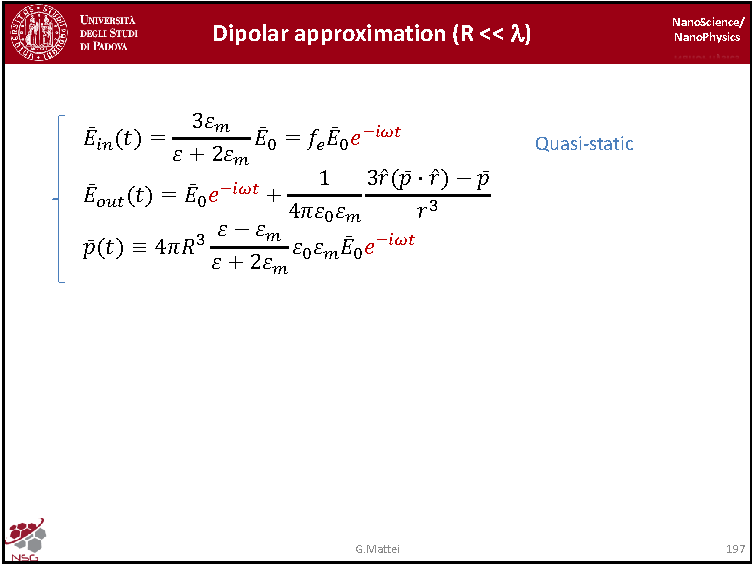
\includegraphics[page=1,width=0.9\textwidth]{../lessons/pdf_file/12_lesson.pdf}
\end{figure}


What I would like to discuss with you today is the extension to the dynamical case, and that extension is very straightforward in the sense that we can obtain the dynamic solution in the quasi-static regime, that is in a regime in which the field is not completely static but varies in frequency and is constant all over the volume of the particle, so that $E_0$ can assume also a spatial dependency provided that the size of the NP is much smaller than the wavelength we can assume that the variation of the field is negligible over the volume of the particle and so the only variation is due to the time variation, which is triggered by the usual exponential harmonic form.

So the solution is straightforward, it is sufficient to just add a temporal evolution at the frequency $\omega$ of the pumping field in each expression involving that field. So the internal field starts to be temporal dependant and also the dipolar moment is temporal dependent and all those fields and the dipolar moment are in phase with the external field.


\newpage

\subsubsection{Slide 198}

\begin{figure}[h!]
\centering
\includegraphics[page=2,width=0.9\textwidth]{../lessons/pdf_file/12_lesson.pdf}
\end{figure}

So, if we look at the near field properties, we can summarize the results that we have obtained. I would like to underline that there is no restriction for this theory to be valid as restricted to metallic particles, it holds whatever is the nature of the NP, provided that the dipolar approximation holds, that is the radius of the particle much smaller than the wavelength.

So I was mentioning that the dielectric function is a complex number and the dielectric function of the medium is a real quantity, so that we can write the dipolar moment, which is function of time, the polarizability $\alpha$ which is of course complex number because $\epsilon$ is complex number, and of course I also underline that any physically measurable quantity is a real quantity, so you need to take the real part of what you are considering, but as you already know from basic physics working whit exponential form instead of trigonometric functions is much more useful so that the derivatives are still in exponential form, whose real or imaginary parts are harmonic functions, so the transition to the general complex notation to the real concept of measurable quantities is straightforward, but it is sufficient to take the real part of the calculated quantity.

The internal field in the idea that we described in the previous lesson, the internal field is the transmitted field $E_t$ is controlled by the local field enhancement and the local field enhancement can be made resonant for specific materials, provided that the Fr$\"o$lich condition is fulfilled, and the Fr$\"o$lich condition is this equation here.

Of course this equation implies that if $\epsilon_m$ is a positive quantity, by definition because it is the square of the refractive index of our materials, and the only solution of this equation can come from materials with a real part of the dielectric function, that is this $\epsilon_1$ strictly negative, and for that reason metallic NP acquired strong interest because metallic NP fulfill this requirement to have a negative real part of the refractive index in the visible or near infrared range, so they can in principle fulfill this equation at least in some specific region of frequencies, whereas normal dielectric materials for sure cannot fulfill this equation because they also have the real part of the dielectric function as positive, so there is no chance to obtain the solution of this equation.

I would like to remind you the close analogy of this Fr$\"o$lich condition with the condition to excite bulk volume plasmon in a metal. You may remember from the Solid State Physics that the condition can be written as the imaginary part of the dielectric function equal to $0$, the value of the frequency at which this equation is satisfied is called bulk or volume plasmon frequency which is related by this equation to the square of the electronic density in our material to other physical constants related to the electrons (charge, mass), and $\epsilon_0$ constant.

Of course in this equation we have an intrinsic property, this is an intrinsic property of that specific material. On the contrary in this equation here you have a combination of the material properties and the environment properties, so the Fr$\"o$lich condition that is the resonance, the localizes SPR condition, is a property of the mixed system, that is the meta-material which is composed by the environment and the metal.

Some straightforward applications of this resonant condition is the fact that if you do inelastic spectroscopy, optical spectroscopy, which is called Raman scattering, is nothing but inelastic scattering of light in which instead of measuring the elastic scattering by the normal processes, you just measure the inelastic component triggered by the absorption into virtual or real states in the nanostructures.

I would not enter into many details of this techniques but normally the cross section, that is the probability of this process to occur, which is normally in the case of inelastic processes very very low, so the probability for this event to occur is much smaller then the elastic scattering. 

But we can enhance the Raman scattering by amplifying the field at the level of the molecule that you want to probe and to investigate, for that reason we speak about surface enhanced Raman scattering, which is kind of flavour of the Raman scattering in which we have an amplification of the field triggered by the presence of a NP, and provided that the Fr$\"o$lich condition is fulfilled, you can have at the level of the surface of our nanostructures an amplification with respect to the incident field $E_i$ which can be as high as one order or even too, in particular condition, with respect to the external phase, so there is a field amplification. 

And since the cross section for the surface enhanced Raman scattering goes like the fourth power of the modulus of the near field, the local field enhancement, you can clearly see that even an amplification of one order of magnitude resolves in an amplification of the efficiency which is of four order of magnitude so quite an interesting process. 

So for that reason ??cells?? had a tremendous development when people realized that you can put the molecules that you want to probe in close proximity to the NP so that the local field provided by the particle is sufficient to amplify the ??cells?? signal.



\newpage

\subsubsection{Slide 199}

\begin{figure}[h!]
\centering
\includegraphics[page=3,width=0.9\textwidth]{../lessons/pdf_file/12_lesson.pdf}
\end{figure}


In this simulation I would like too show a calculation which I will discuss in more detail later, but just to let you see this simple experiment in which we have a silver NP with radius $50 nm$ embedded in silica, this is the cross section of the particle, so dark lines highlight the border of the NP and the scattering geometry in this experiment is like this.    

We have an incident field coming from below and the electric field is polarized in the horizontal direction and what you see here is the vanishing of the local field around the particles, and the colour encodes the intensity of the electric field (blue colour means low intensity and this is the external incident beam, while the red colour on the contrary highlights the region with higher values of the electric field).

The first important result that you can see here is that the field internal to the particle is very high and it is constant all over the volume of the particle and the field also has around the particles a sort of dipolar light character, with these two lobes typical shape f the electric field generated by dipole centered at the center of the NP, and it decays rapidly on moving outside the particle itself, and the region of higher confinement of the field amplification is few nanometers around the particle.

This is an incredible result if you think about the criterion of diffraction limit which is typical of the solution of the Maxwell equation for propagation of electromagnetic excitation, you may remember that when you try to squeeze light in regions much smaller than the wavelengths, light tends to be diffracted, this is the case for example if you have a tiny hole and plane waves transformed into spherical waves, so it is diffracted all over the space.

And there is no chance to force further restraints of space much smaller than half of the wavelength, the is a strong limitation of the solution of electromagnetic problem, but in this case you can clearly see that the NP, in particular a metallic one, which is able to fulfill the Fr$\"o$lich condition because it exhibits a negative refractive index $\epsilon$, you can amplify a lot the external field, so that means you can confine it on sub-wavelengths regions, so this overcoming the diffraction limit in this case.

This is very peculiar phenomenon which has the effect of labeling metallic NP as nano-antenna. A nano-antenna is something which behaves like macroscopic antenna, and an antenna is a device which is able to capture light in resonant way and to reobtain the signal from that wavelength and transform it into readable signal, and a NP is nothing but that, just rescaled down to the domain of the visible range. You may remember that the Maxwell equations are invariant for rescaling the properties of dielectric functions, so it's just controlled by the nature of our materials and if you scale down a typical antenna for radio-waves as length of the waves that is around let's say $1 m$, so for having the very same effect at the nanoscale or in the visible if you want to translate the antenna effect into the visible range, you need to scale down the size of the antenna down to about $10 nm$, so for that reason you are able to couple with the external light and to obtain this nano-antenna effect. I will discuss this later on in this lecture.



\newpage

\subsubsection{Slide 200}

\begin{figure}[h!]
\centering
\includegraphics[page=4,width=0.9\textwidth]{../lessons/pdf_file/12_lesson.pdf}
\end{figure}

Just to give you an example of the local field enhancement, this is a simulation for the silver NP in $SiO_2$ for different values of the radius of the NP, and you clearly see that if you look for instance at $R=10 nm$, we have a very nice resonance as a function of the wavelength of the incoming radiation, and the resonance is around $400 nm$. In this plot I did something that for the moment I cannot explain that is why this function results such dependent? In the previous equation the local field enhancement is not size dependent, so why do we have this effect of the size on the particular value of the field? This is because we need to slightly modify the dielectric function of the metal in order to give better account for the quantum confinement of the electrons in the volume of the NP. So we need to transform the $\epsilon(\omega)$ into $\epsilon(\omega,R)$, and we will see how to do that in a very clever way in the following, but for the moment I would like just to show you how to calculate the modulus of the local field enhancement with this size dependent dielectric function.

But what is important for the moment is the spectral position of this resonance for silver, which is around $400 nm$ and you may remember that this was exactly the resonant wavelength at which we measured the localized SPR in our silver NP obtained by ion implantation in silica, so this is a consistency check.

Another important result here is for instance for the $R=10 nm$ NP, we can obtain value of the modulus of the local field enhancement which exceeds $10$, it is $14$, which is quite nice because if you are able to probe the Raman scattering around this wavelength and you are able to attach a molecule at the surface of your particle, you could obtain an amplification of the Raman scattering cross section, which is $14^4$, so quite nice.




\newpage

\subsubsection{Slide 201}

\begin{figure}[h!]
\centering
\includegraphics[page=5,width=0.9\textwidth]{../lessons/pdf_file/12_lesson.pdf}
\end{figure}


Let's see what happens if you use gold instead of silver: the behaviour is very similar but in this case the local field enhancement is much smaller, we barely go over the value of $2$ which is not bad of course but not as good as silver, for the very same radius. Also in this case I would like to underline the spectral position of the resonance, which is exactly at $535 nm$, in close agreement with what we measured for gold NP in silica obtained by ion implantation, and to understand why we have a much lower field amplification in gold respect to silver we need to better understand how the dielectric function of the two metals differ and how we can describe it quantitatively and possibly size correcting them for obtain this evolution of the field enhancement as a function of the size. 

Another important fact that I would like to Highlight for you is the following: we have this resonance and if you look toward the infrared the resonance goes more smoothly to zero but on the contrary if we go toward the UV the resonance is not symmetric and it stays higher and this difference between the near UV range and the visible or infrared range also can be understood on the basis of nature of complex dielectric function of typical metal like gold or silver, they are both in the group of noble metals but they are different in the dielectric properties as we will see in the following.



\newpage

\subsubsection{Slide 202}

\begin{figure}[h!]
\centering
\includegraphics[page=6,width=0.9\textwidth]{../lessons/pdf_file/12_lesson.pdf}
\end{figure}

So let's look at the way we can use for accessing the Fr$o$lich condition in the visible range for noble metals. If we take our example of gold in silica, we end up in this graph here in which the blue line is the real part of the experimental dielectric function of bulk gold, whereas the red curve here is the imaginary part of the dielectric function of the metal. You clearly see that the real part is largely negative in the near UV and visible range, basically goes to $-\infty$ for typical metals so that for sure you will find a spectral region in which you have negative values. 

We can assume that the dielectric function of $SiO_2$ which is the square of the refractive index is roughly constant over the entire spectral range, this is not the case of course as you may remember from the Cauchy equation, but this assumption is not that strong because the variation of the dielectric function of the other components is much larger, so we can safely assume that the refractive index of silica in the visible range is $1.46$, so the square of that number is this value here, $2.13$, and so to fulfill the Fr$\"o$lich condition we can solve graphically the equation of the Fr$\"o$lich condition that is if we evaluate $-2\epsilon_m$ which amounts at around $4.26$, which is more or less here, and we need to find the matching with the real part of the dielectric function and the interaction occurs  here, which is exactly at the point in which we see the appearance of the resonance.

Of course we have to also look at the imaginary part of the dielectric function because of course the resonance is at that specific position provided that around that value the imaginary part which is at the denominator is not largely varying around the resonance, in this case there is a slight variation but it is not that dramatical, so that we can safely assume that the experimentally measured resonance will occur at this resonance here, but of course this is not the case if the $\epsilon_2$ would vary strongly as a function of the frequency or of the wavelength around the Fr$\"o$lich condition, because this would add small corrections to the Fr$\"o$lich condition for locating quantitatively the experimentally measured resonance, but for a first estimate of the position of the resonance the Fr$\"o$lich condition or the graphical solution of the Fr$\"o$lich condition is an optimal solution.

So you can clearly see that the imaginary part of the dielectric function is not zero, and you see that since the larger is $\epsilon_2$ the larger is the absorption, of course we can say that in the visible and near infrared the absorption is slightly less with respect to the near infrared and UV part of the spectrum, so this portion of the spectrum is controlled by the so called inter-band transition whereas this region here is controlled by the intra-band within the conduction band, you may remember that the noble metals have a Fermi level which is at a half of the conduction band, so metals have a lot of free states above the Fermi level, so this is the intra-band, absorption, and this is the inter-band absorption which triggers the electrons from the valence band toward the conduction band, so the absorption here is larger.

Of course because it took quite larger energy to promote electrons from the valence band towards the conduction band, whereas the energy of those tiny absorption is related to the fact that you have a lot of free states in close proximity to the Fermi level in the metal.

We will get back to the shape of those dielectric functions because we would like to go from this bulk value to a size dependent version of those functions, those are experimentally measured so we can correct to take into account the quantum confinement of the electrons within the volume of the particles.





\newpage

\subsubsection{Slide 203}

\begin{figure}[h!]
\centering
\includegraphics[page=7,width=0.9\textwidth]{../lessons/pdf_file/12_lesson.pdf}
\end{figure}


If we go to the far field properties, so far we spoke about the near field properties and where is the resonant condition for the local field enhancement, but of course the far field properties, which by the way are the quantities that we measure, that is properties that are measured far away from the nanostructure,
far away means at a distance which is much much smaller then the wavelength that we are dealing with, and of course we cannot measure directly the local field around the NP but in general we can simulate it or, under special conditions, also have a measurement of that quantity, that is quite complicated. 

Much easier is to measure the far field properties, that is the properties that we measure in the real world, and in particular the position of the localized surface plasmon resonance is a far field property, because you measure the result of scattering and absorption of incoming light provided that the NP is embedded in a non absorbing medium.

So to arrive to a quantitative description of that specific quantities like cross section for the scattering and absorption of the NP we need to briefly recap what electrodynamics tells us to do when we want to compute the redistribution of energy upon a scattering event. 

If we have plane wave, this plane wave transports energy according to the Poynting vector, that is nothing but the vector product between the electric and magnetic field of the plane wave, and its direction is coincident with the direction of the wavevector of the planewave because of the transversality condition for the field, and the modulus of the Poynting vector is the intensity of the planewave, and dimensions of the Poynting vector are $W/m^2$, it is the energy which passes through the unitary area for the unitary time, so this tells us the intensity of the vector. 

You may notice this prime here that will be clear in a moment, this is the strict definition, but since this is a strong function of time of course if the frequency of our fields is in the visible range, typically we are dealing with hundreds of $THz$ of frequency, so you have a very high number of oscillation per second, so instead of considering the time dependent version of the pointing vector, it is better t consider the temporal average of that Poynting vector, which is basically the average over the period of oscillation $T$ of the harmonic fields in the period, that is $1/T$ times the integral from zero to $T$ of the Poynting vector in $dt$. 

But let's get back to other important equations controlled by classical electrodynamics. You can obtain as a continuity equation for the energy density in the system, that is the temporal variation of the energy density which is defined here is related to the divergence of the Poyning vector, which is also related to the free charge current times the electric field, since we are dealing with no free charges because we have all the neutral systems in which the charges are just those of the NP so free electrons and the positive background of ions cores, in our case this term is zero and so we have this continuity equation for the energy density.

As I mentioned the intensity of the waves is nothing but the modulus of the Poynting vector and as I mentioned previously when we are dealing with measurable quantities of course we need to take the real part of the complex quantities that we normally use to describe fields and vectors in electrodynamics, because only the real quantities can be measured in the real world. 

So if we remind this two remarks we can define the temporal average Poynting vector which is nothing but the average over the period of oscillation of the harmonic field divided by the period, which can read straightforwardly as one half the real part of the cross product between the complex electric fields and the complex conjugate of the magnetic field in complex form.

As we have seen we can decompose all the fields in terms of the outer fields and inner fields inside the particles, so also the Poynting vector can be decomposed in the same very way, as reported in those equations here, and the Poynting vector, which is $S_{out}$ can be written according to this definition in the real version of it, as the real part of the two fields outside the NP, since we want to measure what is emerging from the NP in the far field, this at a large distance from the NP, we are primarily interested in computing the $S_{out}$, which can give us informations about the power scattered in single unit of solid angle around the direction of motion of the incoming beam.

And of course since the outer fields can be decomposed in incident field and scattered field, both for the electric and magnetic part like in this case, if we apply the distribution property of vector product, we can obtain three components of the Poynting vector outside the NP, one which is controlled by the incoming fields, one controlled exclusively by the scattered field and one which is controlled by a mixture of the two electric incoming field and scattered magnetic field an vice versa in this term here.

So basically we can rewrite the Poynting vector outside the particles as the sum of the Poynting vector of the incoming beam plus the Poynting vector of the scattered field plus this additional contribution which is the mixed contribution, that we will label as Poynting vector extinction $S_{ext}$.



\newpage

\subsubsection{Slide 204}

\begin{figure}[h!]
\centering
\includegraphics[page=8,width=0.9\textwidth]{../lessons/pdf_file/12_lesson.pdf}
\end{figure}


So let's see how we can compute all those quantities. The problem is largely simplified by the fact that we are considering a NP in non absorbing medium, so this will give us the freedom to choose the surface over which we can calculate the fluxes by choosing whatever surface at whatever distance we want with respect to the original particle that we located at the origin of our reference frame. 

If we label this surface as a spherical surface with $\Sigma$ we can immediately define which is the net electromagnetic energy flux entering $\Sigma$ and this is indicated with $W_{in}$ (incoming) which is nothing but the flux of the Poynting vector outside the NP, which you may remember is defined by the integral over the surface of the vector of which you want to compute the flux, then you have the scalar product between the local normal to the small element of area $d\Sigma$, so basically if we look at just this quantity here this is the flux by convention the local normal is oriented outside the surface, so if we put a minus in front of this quantity we obtain exactly what we want that is the net electromagnetic energy flux entering $\Sigma$, that is the net energy flux which is trapped into this surface.

And which is the driving force for this trapping of energy? Is the absorption on the NP, so we can be sure that this quantity here is a positive quantity if there is absorption at the NP, of course we do not consider the case in which we could have production of energy inside $\Sigma$, so we have just absorption and since the environment is non absorbing, the only absorption can occur at NP level, so this quantity here should be positive and we can also label that as $W_a$ that is $W$ with absorption like in this situation here.

But of course we can decompose the Poynting vector outside the particle in three terms that we have seen so that we can also decompose this $W_a$ into a sum of three terms which are $W_{i}$ incident, $W_{s}$ scattered and $W_{ext}$ extinction.

Of course this minus sign will be clear in the following. By definition $W_i$ is nothing but minus the integral, just applying the definition and decomposing the value of the Poynting vector outside the NP by highlighting just the contribution to the Poynting vector coming from the incoming beam.

If we just look at this equation here, if the medium is non absorbing and since the incoming field is that you can find also outside the $\Sigma$ surface, of course you end up in the fact that you have the same flux entering and the same flux exiting, so the global result of the integral should be zero provided that the medium is non absorbing, so we have the freedom to choose the distance between the origin and the surface of our $\Sigma$ surface. So if the medium is non absorbing this term should be equal to zero.

The other contribution comes from the $W_s$. This comes from the second term and since by definition the energy of this field is going far from the particle, because it is a scattered field, if we use this minus in front of this definition here, we recover the coherent definition of the flux, in which both $S$ and $u$ are oriented outward with respect to the surface. So for that reason we use this minus here to highlight that this term now is positive.

And the final term, which leaves since it is the $W_{ext}$, so of course using the fact that $W_i$ is exactly zero for non absorbing medium, we can recast this equation here into this equation here in which we have $W_{abs}=-W_{sca}+W_{ext}$. If we move this quantity on the left-hand side of the equation we have a sort of conservation of power, in the sense that the power absorbed by NP plus the power scattered by the NP is what we call the power related to extinction, that is the extinction is nothing but the sum of two processes, the absorption at the NP level and the scattering provided by the NP of the incident energy coming from the planewaves. 

Of course those quantities are clearly units of those $W$s are the units of the Poynting vector times an area, so basically since this is $W/m^2$, the units of those quantities are $W$, this is a power, but of course these values depend on the incoming power, so it is better to normalize them to the incoming intensity, that is the intensity of the planewave pumping the system, which is $I_i$, so that if we normalize all the quantities of this equation by $I_i$ all those quantities are basically in the units of an area, and are measured in $m^2$.




\newpage

\subsubsection{Slide 205}

\begin{figure}[h!]
\centering
\includegraphics[page=9,width=0.9\textwidth]{../lessons/pdf_file/12_lesson.pdf}
\end{figure}


With this observation we can recast this equation into the definition for the cross sections. Cross section are quantities which tells us the probability of a certain event of scattering to occur, and the units of this cross section are typically areas, so that in this case we have this equation here in which we have extinction cross section is nothing but the scattering cross section plus the absorption cross section, telling us that the extinction process is controlled by two independent processes of scattering and absorption at the NP level.

Of course to understand whether those quantities are large or small, of course we need to normalize them to some peculiar area defining our system. For that reason sometimes instead of speaking of cross sections we will use normalized r adimensional quantities which are called efficiencies, which are nothing but the cross section normalized to the geometrical shadow of our particle.

So imagine you are the planewave pointing toward the NP, you will see the cross section of the particle which is a circle with a radius $R$ and the area of the projected cross section, that is the area of the shadow of the particle is nothing but $\pi R^2$ and so if we normalize the cross section for that area we obtain adimensional quantities like the efficiencies which are now $m^2/m^2$ which is an adimensional quantity, and so you can immediately see if there is an enhancement in the cross section process with respect to the geometrical cross section. 

This is straightforward to understand if you think the NP as a macroscopic object and you imagine to shine a planewave on that particles, basically what you will see is the shadow of the particle projected in the wall, and you will see a shadow which has the same size as the NP, so the probability of extinction the direction of observation is exactly related to the geometrical shadow.

Of course when the particle tends to be of the same size of the wavelength also the scattering event is becoming important and you end up in redefinition of both the absorption and the cross section properties, so that you can immediately understand if at a specific wavelength you will have an enhancement with respect to the geometrical cross section of our problem, so for that reason people use efficiency instead of cross section.

Of course this theory is not depending on the shape of the particle, but it can be recast whatever is the shape of the particle, it could be a sphere, an ellipsoid, a rod, whatever shape you may imagine because those things are based on very simple assumption of non absorbing medium around the particles. If the particle has strange or non symmetric shape it would be difficult to calculate the cross section, but the principle is still valid, what we did is just nothing but the conservation of energy in our system and it will be even more complicated to calculate the geometrical  projection of the shape if it is complicated in the direction of motion, but again this theory is not restricted to spherical NP.



\newpage

\subsubsection{Slide 206}

\begin{figure}[h!]
\centering
\includegraphics[page=10,width=0.9\textwidth]{../lessons/pdf_file/12_lesson.pdf}
\end{figure}


So, if we want to give a translation of these far field properties into something which could be really measured, we need to describe now quantitatively what is the effect of light beam passing through a sample containing NP like in this case. Suppose you shine light with intensity $I_0$ with a given frequency and light passes through the sample  whose thickness is $z$, the direction of propagation of the beam, and you want to measure the intensity coming out from the sample at that specific wavelength crossing a thickness $z$ of the sample.

It is straightforward to calculate the value of this intensity, provided that multiple scattering can be negligible, that is light is scattered just once by the interaction with a single NP. 

If this is the case, so basically there is no interaction of each particle with the scattered field of all the other particles, so each particle interacts just with the incoming beam, this is clearly an assumption which is valid provided that the path traveled by the intensity is small with respect to the wavelength of your incoming beam, but in this case we can write a differential equation which is the variation of intensity by traversing a thickness $dz$ infinitesimally small of the sample is controlled by the intensity arriving in that specific thickness times the probability of interaction which is the cross section of extinction times the volumetric density of NP in the samples.

Of course the larger is the number of particles, the larger is the probability to interact and if we check the units of both sides of this equation the intensity is $W/m^2$, this is the same units so all the other quantities should be adimensional, the cross section is an area, this $z$ is a length, so this product is a volume, $\rho$ is a number divided by a volume, so globally the product of the three quantities is adimensional.

So as far as the units those equations are correct, so we can label the product of the volumetric density times the cross section as the extinction coefficient that is this $\gamma$ here which has two contributions because the $\sigma_{ext}$ has two contributions, one for the scattering and one for the absorption, and the single scattering assumption can be recast in this requirement here in which $\gamma z$ ($z$ is the total thickness of the sample) should be much much smaller than the unit, and with this assumption we can straightforwardly solve this equation by separation of variables, so we divide by $I$ and the solution is clearly an exponential decay in which the intensity emerging at specific wavelength traversing a thickness $z$ is the incoming intensity which is exponentially dumped by this coefficient here, since $\gamma$ is a positive quantity, $z$ is a positive quantity, so this is a decreasing quantity.

And we define the trasmittance as the outcoming intensity divided by the incoming intensity, so it is just this exponential factor here so trasmittance is restricted from $0$ to $1$. We could define also the percentage of trasmittance, so that we can express it from $0$ to $100$ as the percentage of light that is transmitted at that specific wavelength.

We can define another important quantity which is the absorbance, which is defined as the logarithm in basis $10$ of the inverse of the trasmittance, basically what we want to obtain is the information on the argument of the exponential function, so you end up with this constant  here, $log_{10}e$. 

Of course a much better definition would have been using the natural logarithm but for historical  reasons people prefer to use the basis $10$, so we need also to consider this constant here, and inserting the explicit form of the $\gamma$ extinction coefficient we end up in the absorbance which is nothing but linearly proportional to the cross section, which is by the way the only quantity which is spectrally dependant on the frequency, on the wavelength, whereas all the other quantities are basically constants and sample dependent ($z$, $\rho$).

So measuring the absorbance is a way to measure the extinction cross section, so this is a very important quantity and it will be used, and actually what we measure when we do the experiment is this quantity here, actually the device which is able to measure those quantity, that is the spectro-photo-meter measures the trasmittance bu it is straightforward to pass from this to the absorbance, and has direct access to the cross section of extinction.





\newpage

\subsubsection{Slide 207}

\begin{figure}[h!]
\centering
\includegraphics[page=11,width=0.9\textwidth]{../lessons/pdf_file/12_lesson.pdf}
\end{figure}







\clearpage


\end{document}